The previous sections show that we can construct hub labels for solving CSP whose preprocessing time, storage and query time can all be parameterized in terms of the constrained highway dimension $h_c$. 
This, however, still does not give a sense of how much worse the hub labels for the CSP problem can be in comparison with those for finding shortest paths. 
We now try to understand this question.
Comparing the size of the \emph{optimal} hub labels for SP and CSP is infeasible as even finding the optimal hub labels for SP is NP-hard~\cite{babenko_hl_complexity}. 
However, since we can parametrize the complexity of HL construction for SP in terms of the HD, a natural question is whether graphs with small HD also have a small CHD. 
Note that the answer to this depends on both the graph and the costs.
We now show that the CHD and, moreover, the sparsity of any EPHS, can be \emph{arbitrarily worse} than the HD. 
\begin{figure}
\begin{center}
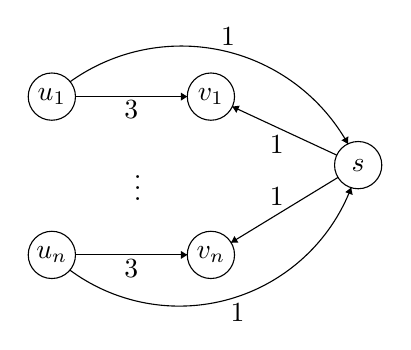
\begin{tikzpicture}[scale=0.1]
\tikzstyle{every node}+=[inner sep=0pt]
\draw [black] (18.5,-12.8) circle (3);
\draw (18.5,-12.8) node {$u_1$};
\draw [black] (38.7,-12.8) circle (3);
\draw (38.7,-12.8) node {$v_1$};
\draw [black] (18.5,-32.9) circle (3);
\draw (18.5,-32.9) node {$u_n$};
\draw [black] (38.7,-32.9) circle (3);
\draw (38.7,-32.9) node {$v_n$};
\draw (29.4,-23.4) node {$\vdots$} ;
\draw [black] (57.4,-21.5) circle (3);
\draw (57.4,-21.5) node {$s$};
\draw [black] (21.5,-12.8) -- (35.7,-12.8);
\fill [black] (35.7,-12.8) -- (34.9,-12.3) -- (34.9,-13.3);
\draw (28.6,-13.3) node [below] {$3$};
\draw [black] (21.5,-32.9) -- (35.7,-32.9);
\fill [black] (35.7,-32.9) -- (34.9,-32.4) -- (34.9,-33.4);
\draw (28.6,-33.4) node [below] {$3$};
\draw [black] (20.825,-10.907) arc (125.59934:29.18714:24.243);
\fill [black] (56.1,-18.8) -- (56.15,-17.85) -- (55.28,-18.34);
\draw (40.87,-6.38) node [above] {$1$};
\draw [black] (56.513,-24.364) arc (-20.88164:-126.45095:23.371);
\fill [black] (56.51,-24.36) -- (55.76,-24.93) -- (56.7,-25.29);
\draw (42.07,-39.01) node [below] {$1$};
\draw [black] (54.84,-23.06) -- (41.26,-31.34);
\fill [black] (41.26,-31.34) -- (42.2,-31.35) -- (41.68,-30.5);
\draw (47.05,-26.7) node [above] {$1$};
\draw [black] (54.68,-20.23) -- (41.42,-14.07);
\fill [black] (41.42,-14.07) -- (41.93,-14.86) -- (42.36,-13.95);
\draw (47.07,-17.66) node [below] {$1$};
\end{tikzpicture}
\end{center}
\caption{Graph with small HD but large CHD: The graph comprises $2n+1$ nodes, with the edge labels representing the lengths. Note that the shortest paths in the graph are of the form $sv_i$, $u_is$ and $u_isv_j$ (for all combinations $i,j$). Thus, the HD is $1$ as $H_{v,r}=\crl{s}$ is a hitting set for all these paths. On the other hand, if we have costs such that $c(u_iv_i)=0\,\forall\,i$, while all other edges have cost $1$, then we have $n$ parallel efficient paths $u_iv_i$, which must all be hit by any EPHS.}
\label{fig:big_chd}
\end{figure}
\begin{proposition}\label[proposition]{prop:example_bad_chd}
There are networks with HD $1$ where the CHD, and also the sparsity of an EPHS, is $n$.
\end{proposition}
\begin{proof}
Consider the directed graph $G$ defined in Figure~\ref{fig:big_chd}.
It is easy to see that $H_{v,r}=\crl{s}$ is a shortest-path hitting set for every $r>0$ and $v\in V(G)$; hence the HD is $1$.
On the other hand, suppose the costs are such that $c(u_iv_i)=0$ for every $i$, while all other costs are set to $1$.
Note that the $1$-significant efficent paths intersecting the ball $B_s(2)$ are $u_iv_i$, which are all disjoint.
Therefore, the hitting set $H_{s,1}$ must contain at least $n$ elements. Moreover, the same argument shows that the sparsity of the best LSHS for $\PS$ is $1$, whereas the sparsity of \emph{any} EPHS is also lower bounded by $n$.
\end{proof}

\begin{remark}
One criticism of the graph in \cref{fig:big_chd} is that it has a maximum degree of $n$.
However, the result holds even for bounded degree graphs.
See \cite{TechReport} for a more involved example showing this.
%In \cref{app:generalhd}, where we discuss alternative notions of HD, we give a more involved example with bounded degrees that exhibits the same separation between LSHS and EPHS for even stronger notions of HD.
\end{remark}

Intuitively, the separation between HD and CHD (or more particularly, the hub labels for computing SPs and CSPs) occurs due to the fact that, for arbitrary graphs and cost functions, the shortest and efficient paths may be completely unrelated. 
For real-world networks, however, this appears unlikely.
In particular, intuition suggests that efficient paths largely comprise of segments which are in fact shortest-paths in their own right. 
This notion can be formalized via the following definition of a \emph{partial witness} 
\begin{definition}[Partial Witness]
Let $\beta\geq 0$.
We say that a path system $\calQ$ is $\beta$-witnessed by the path system $\calQ'$ if, for every $Q\in\calQ$, $\exists Q'\in\calQ'$ such that $Q'\subseteq Q$ and $\ell(Q')\geq 2^{-\beta}\ell(Q)$.
\end{definition}
We can now ask if the hub labels for computing SPs and CSPs can be related in settings where the shortest-path system $\PS$ is a partial witness for the efficient path system $\PE$.
At an intuitive level, the partial witness property says that efficient and shortest paths are not completely different, i.e., if $Q$ is efficient, a fraction $2^{-\beta}$ of $Q$ is a SP.
As a consequence, a node hitting numerous paths in $\PS$, should also hit many paths in $\PE$.
Note that asking for the witness property to hold for all lengths is too extreme, as this essentially requires that all single-hop paths with 0 costs are shortest paths.
Thus, we want this property only for `long-enough' paths. 

We now show that if, for some $\beta$, the network indeed has the partial witness property for paths longer than some $r_\beta$, then we can relate the HL sizes for the two problems in terms of $\beta$ and the doubling dimension $\alpha$. 
Note that the doubling dimension depends on $G$ and $\ell$; the partial witness property depends on the interplay between $G$, $c$ and $\ell$.
Observe also that, if $\alpha$ is a constant, then the requirement in \cref{theo:witness_doubling} is for paths longer than $r_\beta\sim h\alpha^{\beta-2}$.
\begin{theorem}\label{theo:witness_doubling}
Assume $G$ is $\alpha$-doubling and $\PE_r$ is $\beta$-witnessed by $\PS$ for every $r\geq r_\beta$, where $r_\beta=2^{\log_\alpha(\alpha^{\beta-2} h)}$. 
Then, for any $r>0$, given an $(h,r)$-LSHS, we can construct, in polynomial time, an $(\alpha^{\beta} h,r)$-EPHS for $(G,\ell,c)$. 
\end{theorem}

\begin{proof}
For any $r$, we need to construct a hitting set $C^E$ for $\PE_r$.
Assume first $r\geq r_\beta$.
Take $C$ as the hitting set for $\PS_{2^{-\beta}r}$, which is guaranteed to be sparse with respect to balls of radius $2^{-\beta+1}r$.
Define the desired set by
\[
C^E\defeq\{v\in C: v \text{ is in some $r$-efficient path} \}.
\]

Since $\PS$ is a $2^{-\beta}$-witness for $\PE_r$, $C^E$ is indeed a hitting set for $\PE_r$.
We are only left to prove the sparsity.
Take some $u\in V$, by doubling dimension we can cover $\Bf_{2r}(u)$ by at most $\alpha^\beta$ balls of radius $2^{-\beta+1}r$.
Each of these balls contains at most $h$ elements of $C$, therefore the sparsity is as claimed.
The argument for reverse balls is identical.

Now we analyse the case $r< r_\beta$.
It is no longer true that efficient paths are witnessed, but now the neigborhoods are small.
We first claim that, for any $v\in V$ and $r>0$, $\abs{B_{r}(v)}\leq \alpha^{\log_2r+1}$.
Indeed, using the doubling property $\log_2r+1$ times, we can cover $B_r(v)$ with balls of radii $1/2$.
Since the minimum edge length is $1$, all of these balls must be singletons and the claim follows.
Now we can take $C=V$ as the EPHS.
Clearly $C$ hits all the paths and the local sparsity is at most the size of the ball.
Using our assumption on $r_\beta$, a simple computation shows that $\card{B_{2r}(v)}\leq \alpha^{\log_2r_\beta+2}\leq h\alpha^\beta$. 
\end{proof}
\begin{remark}
The existence of a $\beta$-witness is not enough to bound the CHD. 
Nevertheless, as we discuss in Section~\ref{ssec:hldef}, the existence of $(h,r)$-LSHS already allows the construction of HL. 
%Moreover, the above argument does indeed give a bound for a weaker definition of HD (details in \cite{TechReport}).
\end{remark}
%\begin{remark}
%In order to make it more transparent, we state the above result in terms of $\alpha$ and $h$. 
%However, these quantities are somewhat related; it can be shown that $\alpha\leq 2h\Delta+1$ (cf.~\cite{skeleton}).
%\end{remark}